\documentclass[a4paper,12pt]{article}


\usepackage[utf8]{inputenc}
\usepackage[Italian]{babel}
\usepackage{amsmath}
\usepackage{amsfonts}
\usepackage{amssymb}
\usepackage{graphicx}
\usepackage{hyperref}
\usepackage{minted}
\usepackage{geometry}
\geometry{a4paper, margin=1in}
\hypersetup{colorlinks,urlcolor=blue}

\title{Relazione di Elettronica}
\author{Andrea Boldetti}
\date{\today}

\begin{document}

\maketitle

\begin{abstract}
Inserisci qui il riassunto del documento.
\end{abstract}

\newpage
\tableofcontents

\section{Introduzione}
Inserisci qui l'introduzione.

\section{Microcontrollore}
\subsection{Funzionamento generale}

\subsection{GPIO}

\subsection{USART}

\subsection{ADC}

\subsection{DMA}

\subsection{DAC e Comparatore}

\pagebreak
\section{Scheda Analogica}
\textbf{Lavoro di Gruppo:   Yehan Edirisinghe,  Andrea Boldetti,    Elisa Minelli}

In questa sezione viene discussa la caratterizzazione degli Amplificatori Operazionali e il loro utilizzo all'interno della scheda analogica fornita:

\begin{figure}[!h]
    \centering
    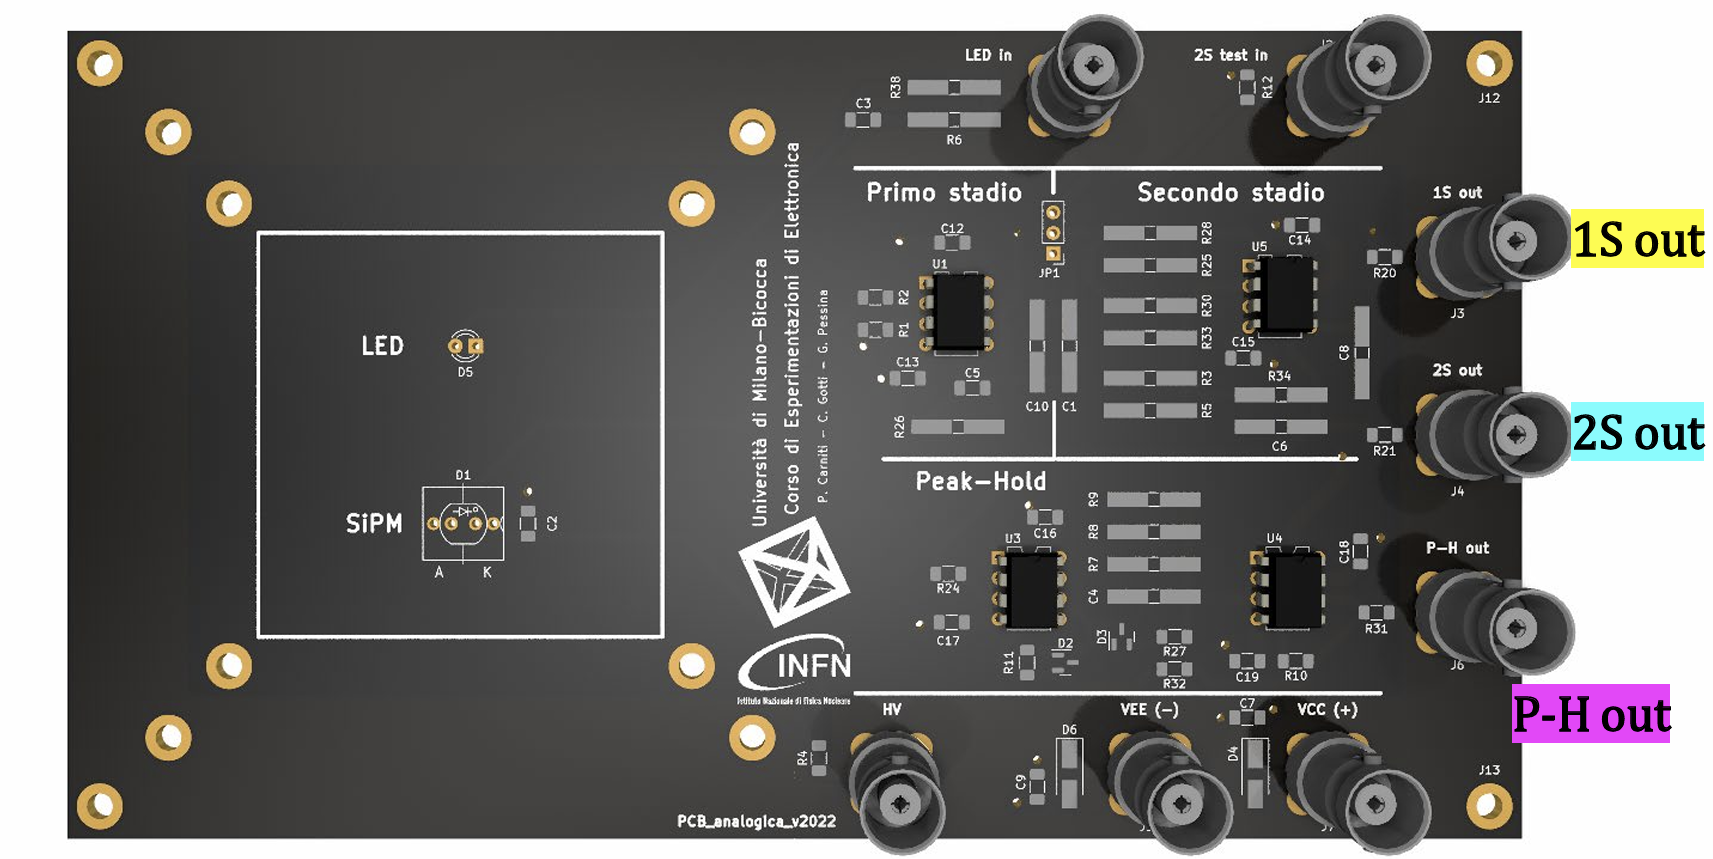
\includegraphics[width=0.5\linewidth]{analog/assets/scheda analogica/Scheda_Analogica.png}
    \caption{Scheda Analogica}
\end{figure}

Il nostro obbiettivo è rendere il segnale uscente da un SiPm a stato solido leggibile dall'ADC del microcontrollore. Siccome la risposta del sensore ad un fotone è a tensioni troppo basse per la risoluzione dell'ADC, è necessario implementare degli stadi di amplificazione.

\paragraph{Nota}
Per le funzioni di trasferimento degli amplificatori è stata fatta la seguente semplificazione:

\begin{figure}[!h]
    \centering
    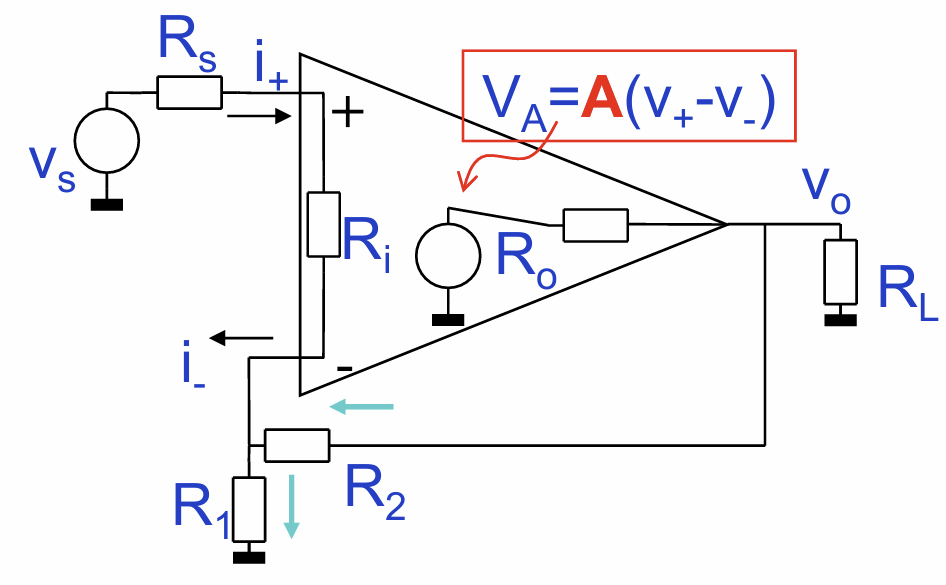
\includegraphics[width=0.5\linewidth]{analog/assets/scheda analogica/T(s)_Approx.png}
    \label{fig:enter-label}
\end{figure}

\[ T = -\frac{R_i}{R_s + R_i} \frac{AR_1}{R_1 + R_2} \frac{R_L}{R_o+R_L} \sim -A\beta \]

Questo è accettabile siccome la resistenza del generatore è stata impostata a $R_s \sim 50\Omega$ e $R_L \sim 1M\Omega$.

\pagebreak
\subsection{OP27}

\begin{wrapfigure}{R}{.4\linewidth}
    \centering
    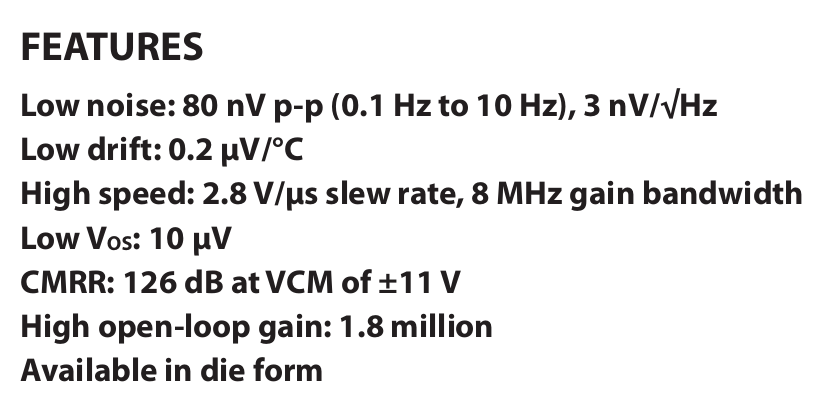
\includegraphics[width=\linewidth]{assets/OP27/OP27_datasheet.png}
    \caption{Feature OP27}
\end{wrapfigure}

Il primo amplificatore che vogliamo studiare è l' OP27 che dai datasheet risulta essere un amplificatore a singolo polo dominante ovvero della forma:
\[A(s) = \frac{A_o}{1+s\tau_A}\]
Le cui caratteristiche sono descritte in dettaglio nei datasheet.



In particolare è segnata una \textbf{Bandwidth} di circa \textbf{8Mhz} che risulterà essere il dato di nostro interesse.

L'amplificatore può essere configurato in due modalità, ovvero: configurazione
invertente e configuraizone non invertente come mostrato in figura:

\begin{figure}[!h]
    \centering
    \begin{subfigure}[b]{0.45\textwidth}
        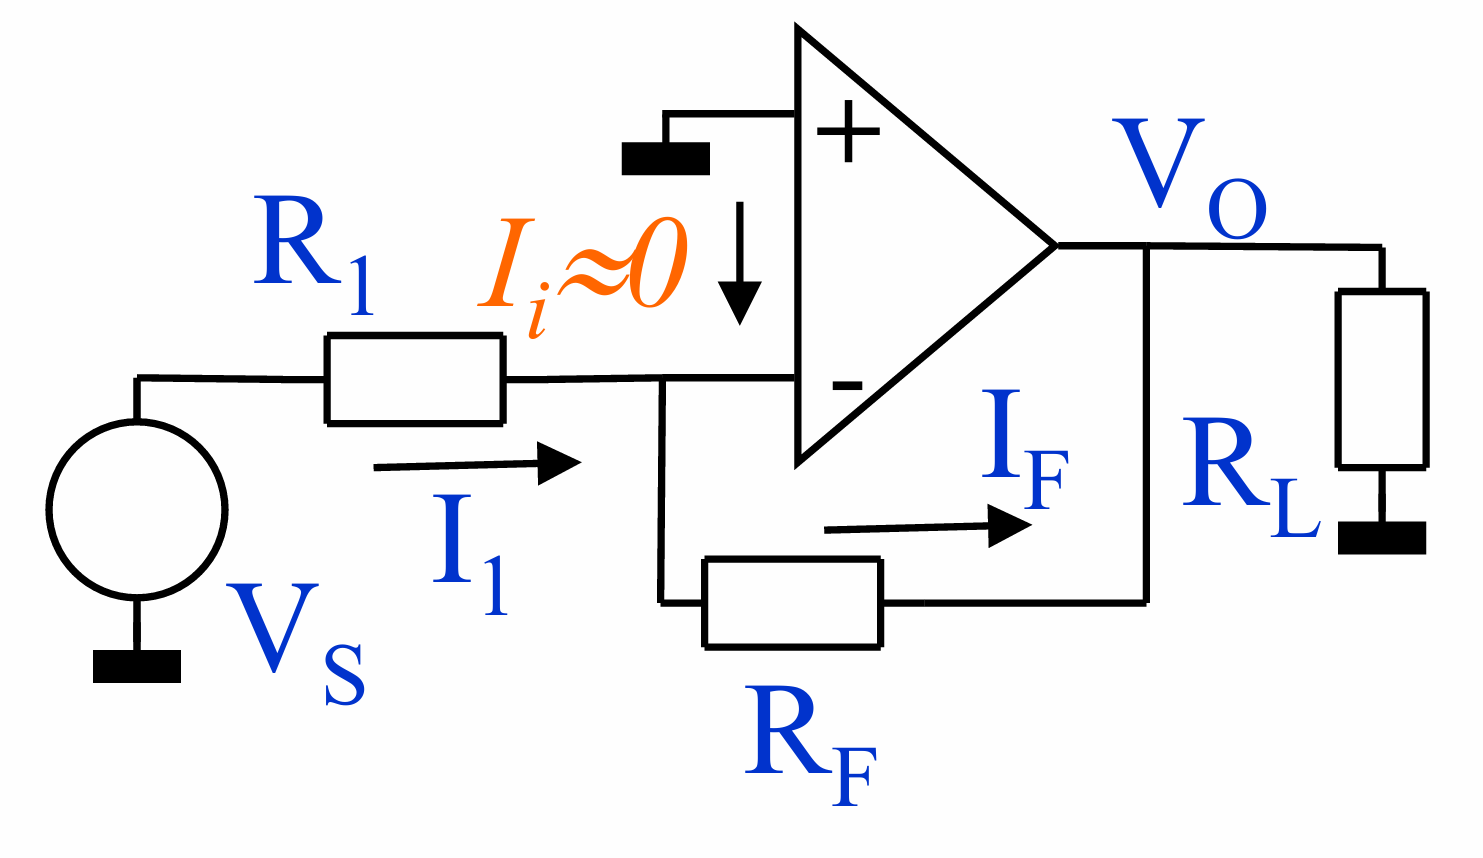
\includegraphics[width=0.9\textwidth]{assets/scheda analogica/invertente.png}
        \caption{configurazione invertente}
    \end{subfigure}%
    \begin{subfigure}[b]{0.45\textwidth}
        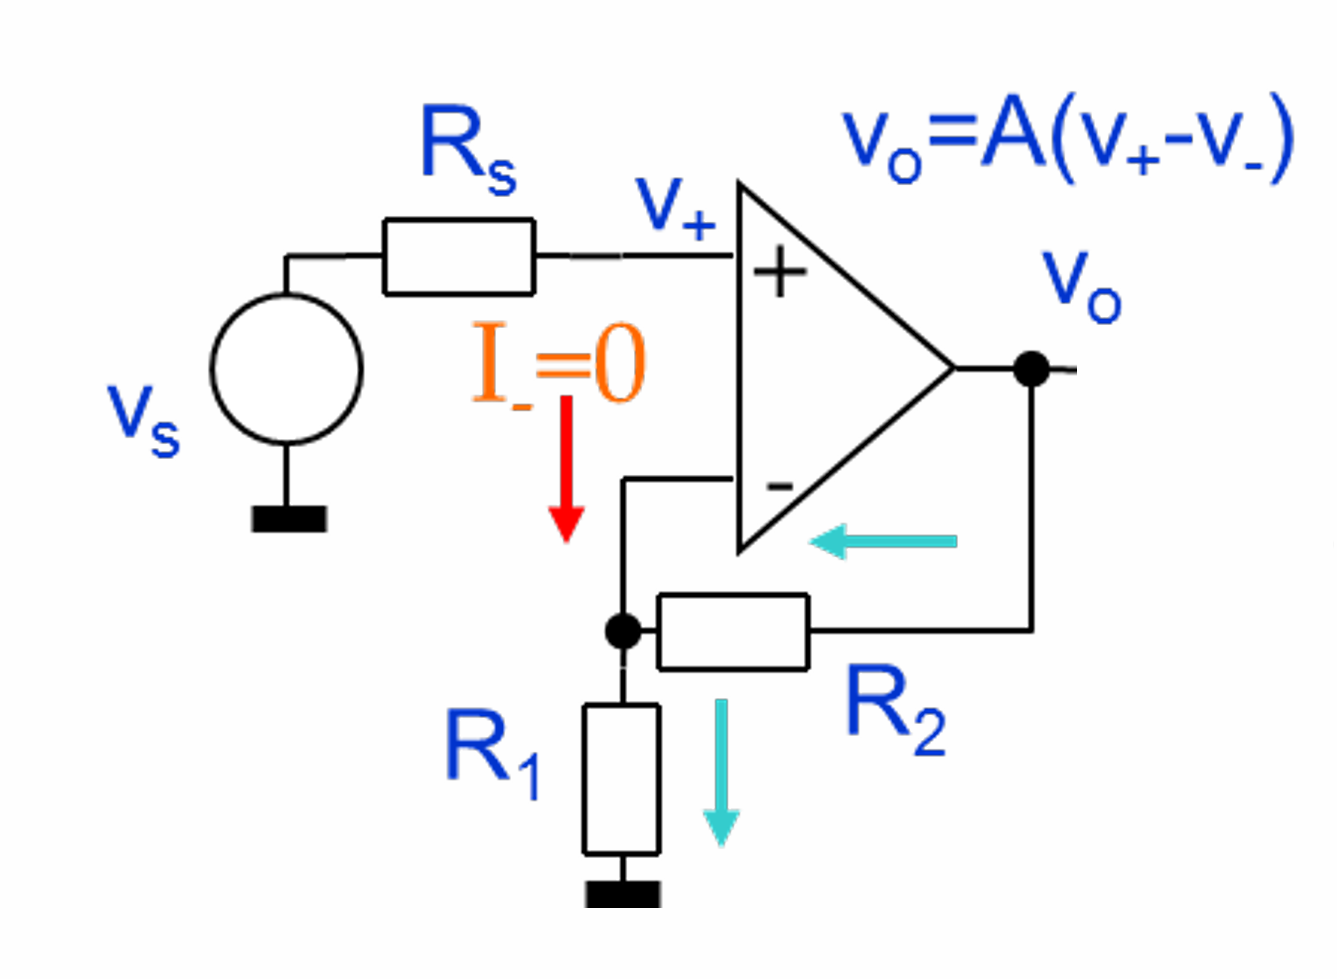
\includegraphics[width=0.9\textwidth]{assets/scheda analogica/non_invertente.png}
        \caption{configurazione non invertente}
    \end{subfigure}
\end{figure}

Queste risultano entrambe utili a seconda dello stadio di amplificazione. La configurazione invertente permette un guadagno maggiore a costo di invertire il segnale.
La configurazione non invertente invece non altera il segnale ma applica semplicemente un'amplificazione.

\subsubsection{Configurazione Non Invertente}

In questa configurazione abbiamo un guadagno di Gain $\frac{1}{\beta} = \frac{R_1+R_2}{R_1}$ nel caso di amplificatiore \textbf{ideale}.
Collegando nella scheda resistenze $R_s = 0.5 \Omega$, $R_1 = 2.2k\Omega$ e $R_2 = 2.2k\Omega$ ci aspettiamo un gain di 2.

Siccome l'amplificatore reale dista dal modello ideale di un polo complesso, è necessario considerare il fattore $\frac{A(\omega)}{\beta}$ al posto di $\frac{1}{\beta}$ nella sua funzione di trasferimento dove A($\omega$) denota la dipendenza dalla frequenza. Per poter caratterizzare questo comportamento in frequenza vogliamo trovare la \textbf{banda} dell'amplificatore.

\'E possibile utilizzare tre modalità diverse:
\begin{enumerate}
    \item Analisi di onde sinusoidali
    \item Analisi su un'onda quadra
    \item Analisi dello spettro
\end{enumerate}

\paragraph{Analisi sinusoidale con $R_1=2.2k\Omega$ e $R_2=2.2k\Omega$:}

Per questa modalità è stato impostato un segnale sinusoidale all'ingresso non invertente dell'OP27 ad una ampiezza nota e osservato tramite oscilloscopio la risposta del circuito nel dominio del tempo alle varie frequenze. Per il calcolo della banda è sufficiente trovare la frequenza per cui il gain diminuisce di 3dB, ovvero perde il 30\% della sua ampiezza.

\begin{figure}[!h]
    \centering
    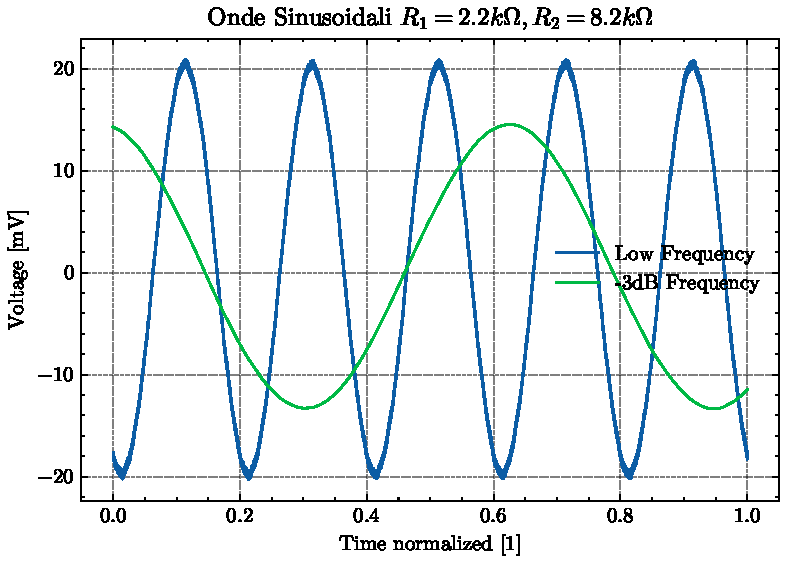
\includegraphics[width=0.5\linewidth]{assets/OP27/Non Invertente/Sin_2k2.pdf}
    \caption{Segnali di uscita dall'amplificatore per frequenza a risposta piatta e a -3dB, (\href{https://github.com/Yedi278/Esperimentazioni-Elettronica/tree/main/-\%20OPAMP/OP27/Non-Invertente/R1\%3D2.2k\%2CR2\%3D2.2k}{link dati})}
\end{figure}

Come frequenza bassa è stato usato un segnale sinusoidale di circa 1KHz mentre la frequenza per cui il segnale perde 3dB è di circa 3.9Mhz.
Per la banda si trova: \bm{$Banda = \frac{\omega_F}{\beta} = 7.8 Mhz$}.

\paragraph{Analisi in onda quadra a $R_1=2.2k\Omega$ e $R_2=2.2k\Omega$:}

Per questa modalità è stata impostata nel generatore un'onda quadra e tramite la modalità di misura dell'oscilloscopio sempre nel dominio del tempo, è stato acquisito il valore di \textbf{rise time} della risposta dell'amplificatore. Con rise time si intende il tempo che impiega il segnale a passare dal 10\% al 90\% della sua ampiezza.

\begin{figure}[!h]
    \centering
    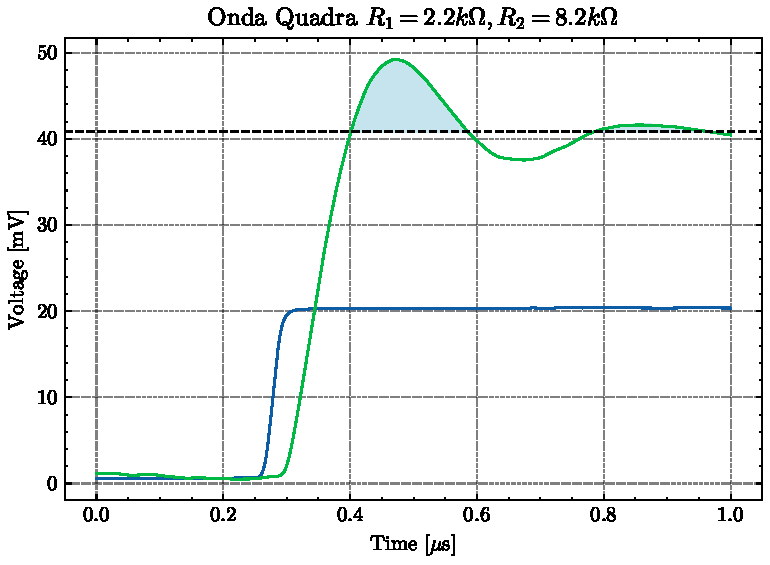
\includegraphics[width=0.5\linewidth]{assets/OP27/Non Invertente/Square_2k2.pdf}
    \caption{Risposta ad onda quadra, (\href{https://github.com/Yedi278/Esperimentazioni-Elettronica/tree/main/-\%20OPAMP/OP27/Non-Invertente/R1\%3D2.2k\%2CR2\%3D2.2k}{link dati})}
\end{figure}
\pagebreak

Il rise time misurato dall'oscilloscopio è di 79.5 ns che corrispondono ad una frequenza a -3dB di:
$$f_{-3dB} = \frac{0.35}{t_r} = 4.4Mhz$$ e dunque una \textbf{banda di 8.8Mhz}.

% \paragraph{Nota}
% \'E possibile notare nella risposta in onda quadra un comportamento insolito, infatti è presente un notevole overshoot (circa 20\%) nella risposta dell'amplificatore.


% Siccome un amplificatore a singolo polo non dovrebbe mostrare questo fenomeno è necessario supporre che la presenza di singolo polo dominante sia errata. Una opzione è quella di considerare anche la presenza di capacità parassite in parallelo alle resistenze del circuito. 

% Tramite le formule presenti nel pdf al \href{https://pessina.mib.infn.it/Corsi_del_III_anno/CorsoStrumentazioneElettronica/Corso_2425/Amplificatori_reazionati_analisi_tempo_frequenza_B_2425.pdf}{link} e discussa più in dettaglio nel file \href{https://github.com/Yedi278/Esperimentazioni-Elettronica/blob/main/Analisi_Overshoot.mlx}{matlab}, si ottiene: 

% \begin{equation}
%     T(s) = \frac{R_1+R_2}{R_1} \frac{1+s\tau_2}{(1+s\tau_1)(1+s\tau_A)} A_o
% \end{equation}

% Dunque si può osservare un andamento a doppio polo che potenzialmente potrebbe portare a spiegare l'andamento ma come mostrato più in dettaglio nel file matlab il valore delle capacità parassite dovrebbe superare notevolmente l'odine dei pico-Farad, che risulta insolito. \'E dunque necessario escludere anche questa possibilità.

% Non resta altro che supporre non trascurabile l'influenza di altri poli all'interno dell'OP27 per frequenze maggiori del polo dominante.


%\textcolor{red}{Bolde}
\begin{flushleft}

\colorbox{notebox}{
\begin{minipage}[]{\textwidth}

    Notiamo come in risposta all'onda quadra, l'amplificatore presenti un'overshoot non trascurabile: circa il 20\% rispetto al valore aspettato.
Questo può essere dovuto a diversi fattori:
\begin{itemize}
    \item la presenza di capacità parassite all'interno dell'amplificatore
    \item la presenza di un secondo polo nell'amplificatore che abbia un influenza inaspettata anche a frequenze basse
\end{itemize}
Prendendo in considerazione l'ipotesi di capacità parassite all'interno dell'amplificatore, si può modificare la formula della funzione di trasferimento come segue
\begin{equation}
    T(s) = \frac{R_1+R_2}{R_1} \frac{1+s\tau_2}{(1+s\tau_1)(1+s\tau_A)} A_o
\end{equation}
Il quale motiva la presenza del doppio polo. Sfortunatamente, questa ipotesi va scartata in quanto dai dati risulta che le capacità dovrebbero essere molto maggiori del pico Farad, il quale risulta insolito.

Risulta quindi la seconda ipotesi, ovvero che l'OP27 non sia accettabile come amplificatore a polo singolo ma è necessario considerare anche i poli di ordine superiore per avere delle misure coerenti con la teoria
\end{minipage}
}
\end{flushleft}



%\textcolor{red}{fine Bolde}


\begin{figure}[!h]
    \centering
    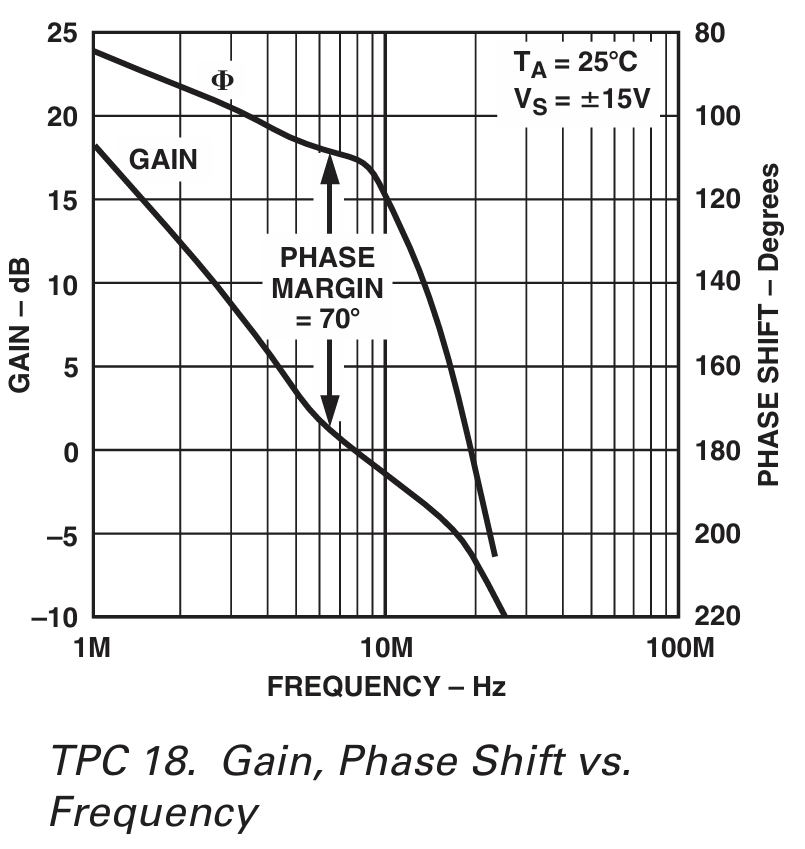
\includegraphics[width=0.3\linewidth]{assets/OP27/OP27_Phase_Margin.png}
    \caption{Matgine di fase OP27}
\end{figure}

\begin{flushleft}
    

\colorbox{notebox}{
\begin{minipage}[]{\textwidth}
Guardando nei datasheet la fase dell'amplificatore si nota che a gain bassi ci si può ridurre nella condizione con margine di fase ridotto. In questa zona possiamo dedurre che si abbiano effetti non previsti come l'andamento instabile osservato nelle misure sperimentali.

Inoltre questa ipotesi a differenza delle altre è consistente con l'andamento osservato per l'overshoot in figura \ref{fig:OP27 overshoot non invertente} che diminuisce all'aumentare del gain assegnato.
\end{minipage}
}
\end{flushleft}
\paragraph{Nota 2}
Siccome in alcuni casi il generatore di onda quadra non risulta perfetto è necessario considerare il rise time di quest'ultimo:
\[t_r = \sqrt{t_m^2 + t_g^2}\]
dove $t_m$ è il rise time misurato e $t_g$ il rise time del generatore da solo.

\pagebreak

\begin{wrapfigure}{R}{.4\linewidth}
    \centering
    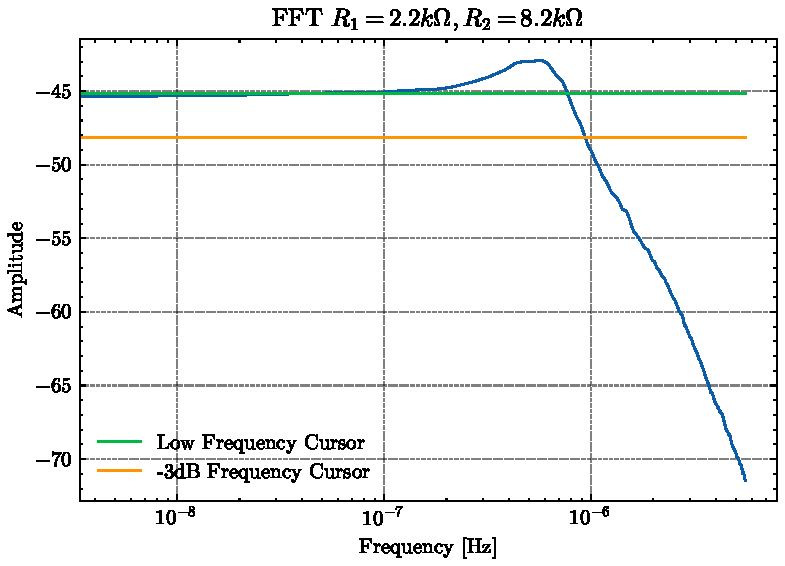
\includegraphics[width=\linewidth]{assets/OP27/Non Invertente/FFT_2k2.pdf}
    \caption{ (\href{https://github.com/Yedi278/Esperimentazioni-Elettronica/tree/main/-\%20OPAMP/OP27/Non-Invertente/R1\%3D2.2k\%2CR2\%3D2.2k}{link dati})}    
\end{wrapfigure}

\paragraph{Analisi Spettrale per  $R_1=2.2k\Omega$ e $R_2=2.2k\Omega$:}
L'ultima misura sfrutta il rumore bianco, ovvero rumore che ha potenza spettrale piatta e dunque uguale a ogni frequenza.
Avendo selezionato nel generatore un rumore bianco, è stata utilizzata la funzione FFT dell'oscilloscopio per ottenere lo spettro dell'amplificatore.





\'E possibile in questo caso utilizzare manualmente due cursori per individuare il gain a risposta piatta e dato questo, individuare la frequenza a -3dB da quest'ultima.


 Nella misura otteniamo una risposta piatta a circa -45dB e una $f_{-3dB} = 3.8Mhz$ da cui una \textbf{banda di 7.6Mhz}.

\paragraph{Cambio Resistenze}
Variando la resistenza $R_2$ è possibile cambiare il gain del circuito e studiare l'andamento della banda.
Ripetendo il processo eseguito prima per valori di $R_2 = \{2.2k\Omega, 8.2k\Omega, 10k\Omega, 17.2k\Omega\}$ è possibile notare il seguente andamento: 

\begin{figure}[!h]
    \centering
    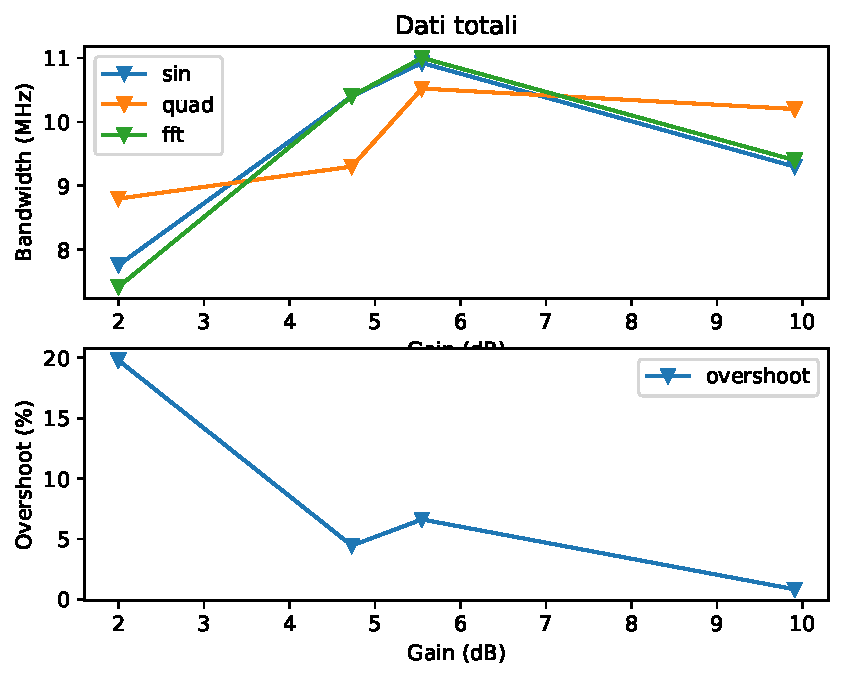
\includegraphics[width=.5\linewidth]{assets/OP27/Non Invertente/Non_Invert_Dati_tot.pdf}
        \captionof{figure}{Rappresentazione grafica dell'andamento per configurazione Non-invertente}
        \label{fig:OP27 overshoot non invertente}
\end{figure}

\begin{table}[!h]
    \centering
    \begin{tabular}{|l|l|l|l|l|}
            \hline
            \textbf{Gain {[}1{]}} & \textbf{Sin {[}Mhz{]}} & \textbf{Square {[}MHz{]}} & \textbf{Fft {[}MHz{]}} & \textbf{Overshoot {[}MHz{]}} \\ \hline
            2             & 7.76         & 8.8             & 7.42         & 19.8               \\ \hline
            4.73          & 10.4         & 9.3             & 10.4         & 4.45               \\ \hline
            5.55          & 10.92        & 10.52           & 11           & 6.62               \\ \hline
            9.91          & 9.3          & 10.2            & 9.4          & 0.83               \\ \hline
        \end{tabular}
        \captionof{table}{Rappresentazione a tabella dei dati per configurazione Non-invertente}
\end{table}

Il valor medio di banda ricavato è di \textbf{9.6MHz}.

\paragraph{Conclusioni}
 \'E stato possibile con tre metodi diversi eseguire un'analisi della risposta del circuito alle frequenze in ingresso. In particolare è stato riscontrato un polo complesso che porta ad una larghezza di \textbf{banda $\sim 9.6$Mhz} che risulta in accordo entro un 20\% con il valore dei datasheet.

\subsubsection{Configurazione Invertente}

L'altra configurazione interessante per un amplificatore è quella invertente in cui il segnale entra nell'ingresso negativo $V^-$.
 In questa configurazione si ha un guadagno di $$Gain = -\frac{R_2}{R_1}$$

 Il procedimento per caratterizzare la banda risulta identico ed è possibile nelle tre modalità citate prima.

 Questo è un esempio di risposta osservato per resistenze di $R_1 = R_2 = 2.2k\Omega$

\begin{minipage}{0.8\textwidth}

    \centering
    \begin{minipage}[b]{0.3\textwidth}
        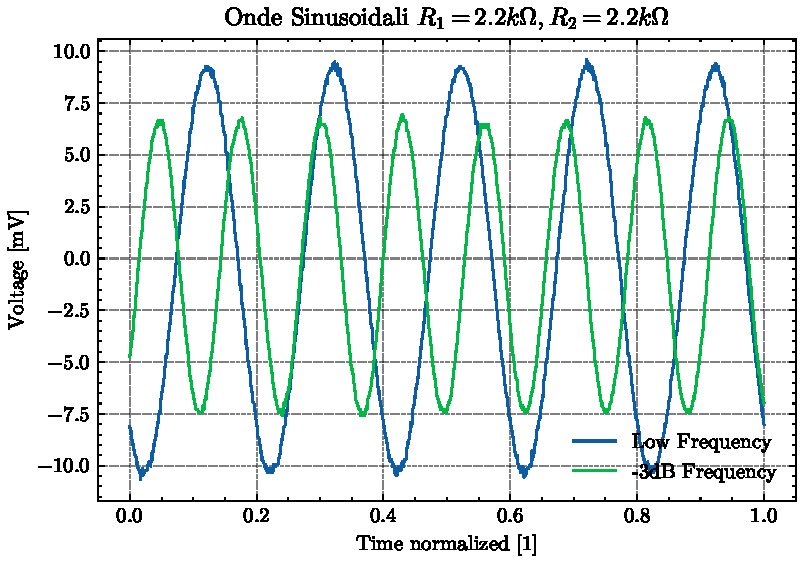
\includegraphics[width=\linewidth]{assets/OP27/Invertente/Sin_17k8.pdf}
        \captionof{figure}{Analisi con segnale sinusiodale}
    \end{minipage}
    \hfill
    \begin{minipage}[b]{0.3\textwidth}
        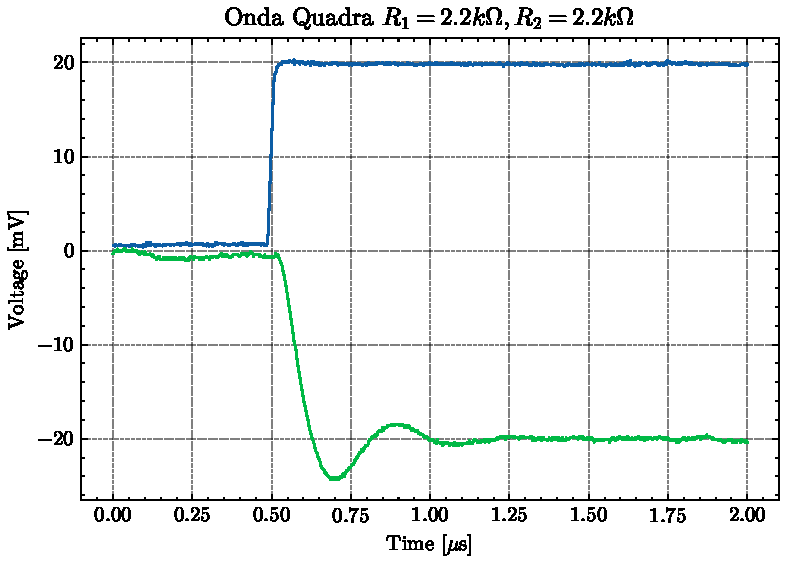
\includegraphics[width=\linewidth]{assets/OP27/Invertente/Square_17k8.pdf}
        \captionof{figure}{Analisi con onda quadra (overshoot $<$ 20\%)}
    \end{minipage}
    \hfill
    \begin{minipage}[b]{0.3\textwidth}
        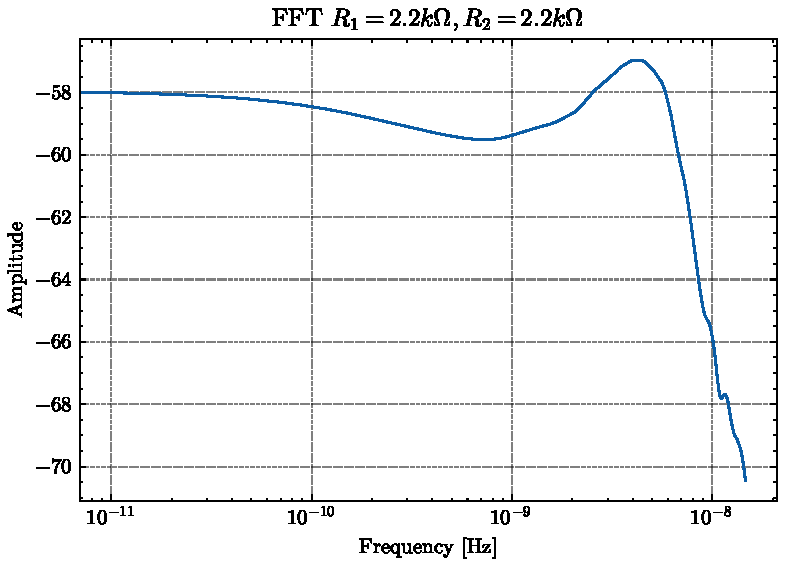
\includegraphics[width=\linewidth]{assets/OP27/Invertente/FFT_17k8.pdf}
        \captionof{figure}{Analisi nel dominio delle frequenze}
    \end{minipage}
    \hfill    
\end{minipage}

Da notare che l'uscita è invertita rispetto al segnale. Il resti dei dati è al link: (\href{https://github.com/Yedi278/Esperimentazioni-Elettronica/tree/main/-\%20OPAMP/OP27/Invertente}{link dati})

\paragraph{Risultato:}
Applicando il processo di misura per varie resistenze $R_2 = \{ 2.2k\Omega, 8.2k\Omega, 10k\Omega, 17.8k\Omega \}$ è possibile vedere l'andamento seguente:

\begin{figure}[!h]
    \centering
    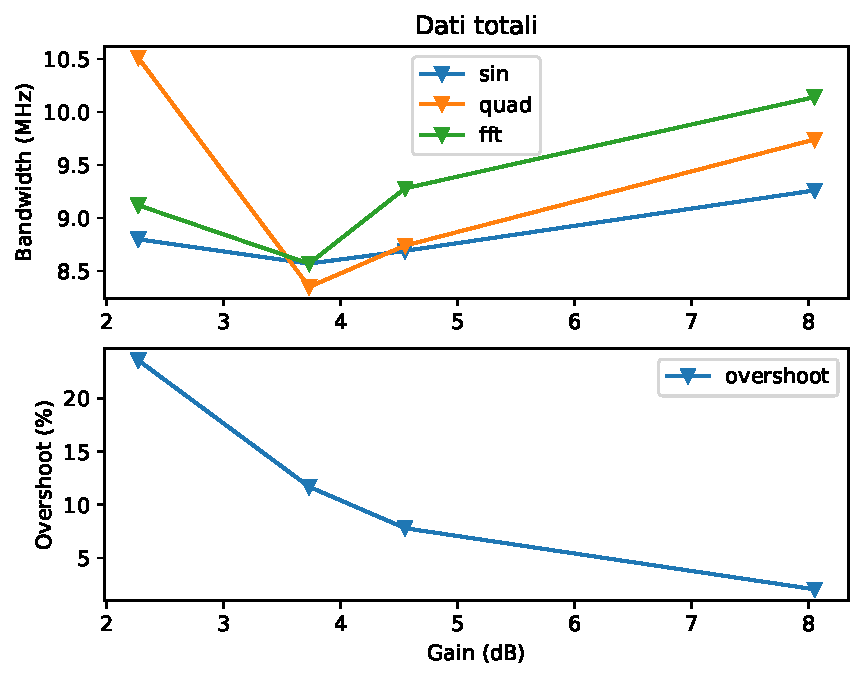
\includegraphics[width=.5\linewidth]{assets/OP27/Invertente/OP27_Invert_Dati_tot.pdf}
    \captionof{figure}{Rappresentazione grafica dell'andamento per configurazione Non-invertente}
\end{figure}

\begin{table}[!h]
    \centering
    \begin{tabular}{|c|c|c|c|c|}
    \hline
    \textbf{Gain {[}1{]}} & \textbf{Sin {[}Mhz{]}} & \textbf{Square {[}MHz{]}} & \textbf{Fft {[}MHz{]}} & \textbf{Overshoot {[}MHz{]}} \\ \hline
    2.27                  & 8.8                    & 10.51                     & 9.12                   & 23.6                         \\ \hline
    3.73                  & 8.57                   & 8.35                      & 8.57                   & 11.7                         \\ \hline
    4.55                  & 8.69                   & 8.74                      & 9.28                   & 7.8                          \\ \hline
    8.05                  & 9.26                   & 9.74                      & 10.14                  & 2.05                         \\ \hline
    \end{tabular}
    \captionof{table}{Rappresentazione a tabella dei dati per configurazione Non-invertente}
\end{table}


Come per il caso non invertente si osserva una diminuizione dell'overshoot all'aumentare del gain nel circuito. 

\subsubsection{Conclusione}

L'unione dei dati presi tramite le due configurazioni porta al seguente andamento:

\begin{figure}[!h]
    \centering
    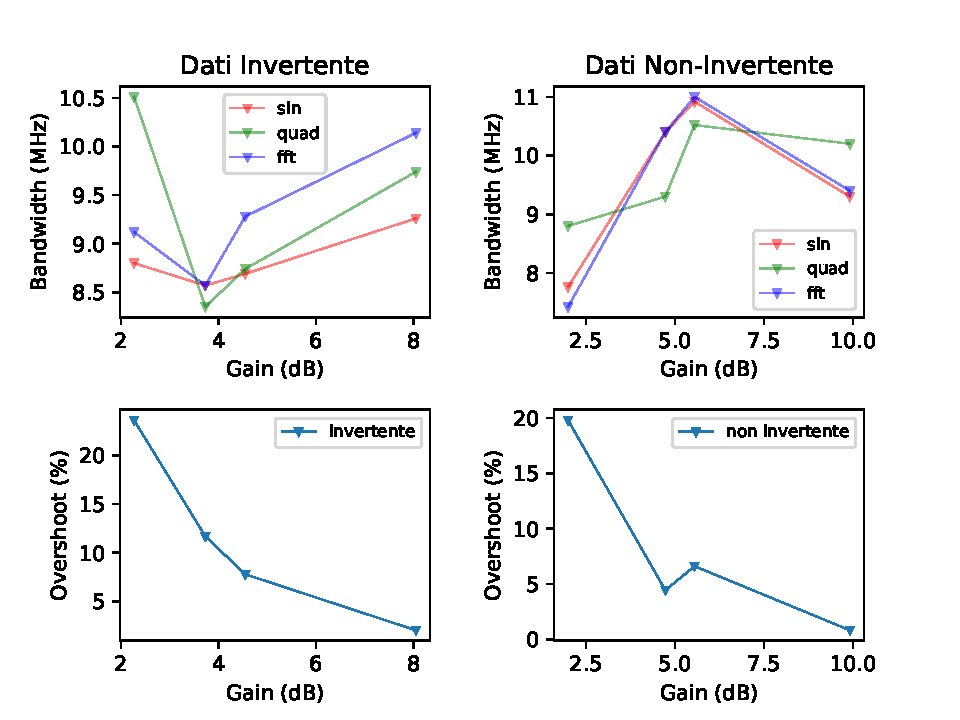
\includegraphics[width=\linewidth]{assets/OP27/Inv+Non-Inv.pdf}
    \caption{Valori di banda calcolati tramite le tre configurazioni per Invertente e Non-inv, (\href{https://github.com/Yedi278/Esperimentazioni-Elettronica/tree/main/-\%20OPAMP/OP27}{link dati})
    }
\end{figure}

\'E possibile notare che tra i due modelli si ottiene lo stesso andamento per l'overshoot che conferma l'ipotesi di dipendenza dai componenti interni all'amplificatore escludendo elementi esterni come capacità parassite.
\'E possibile inoltre notare una dispersione elevata delle misure. Questo si suppone dovuto ad errori di imprecisione nella presa dati (es cursori non perfettamente allineati o resistenze con tolleranze elevate).

Tramite i dati raccolti è possibile ottenere una stima della banda di \textbf{9.4 ± 0.9 MHz}. Il valore di riferimento di 8Mhz entra in 1.5 $\sigma$ dalla stima.



\newpage

\subsection{AD848}

Il nostro obbiettivo finale è la caratterizzazione degli amplificatori AD848 che verranno tenuti nella configurazione finale della scheda analogica.
Questo amplificatore a differenza dell'OP27 è garantito nei \href{https://www.analog.com/media/en/technical-documentation/data-sheets/AD848.pdf}{datasheet} con un gain minimo di 5. In questa sezione vogliamo eseguire una caratterizzazione della sua banda e indagare la zona a basso gain.

\subsubsection{Oscillazioni a Gain BASSO}

Montando l'amplificatore nella configurazione non invertende, come visto in precedenza, abbiamo un gain di $$\frac{1}{\beta} = \frac{R_1+R_2}{R_1}$$ per cui utilizzando resistenze $R_1 = 2.2k\Omega$ e $R_2 = 2.2k\Omega$ si ottiene un gain di 2 che risulta essere inferiore alla soglia di 5 per il funzionamento prescritto nel manuale.

\begin{figure}[!h]
    \begin{minipage}{.5\linewidth}
        \centering
        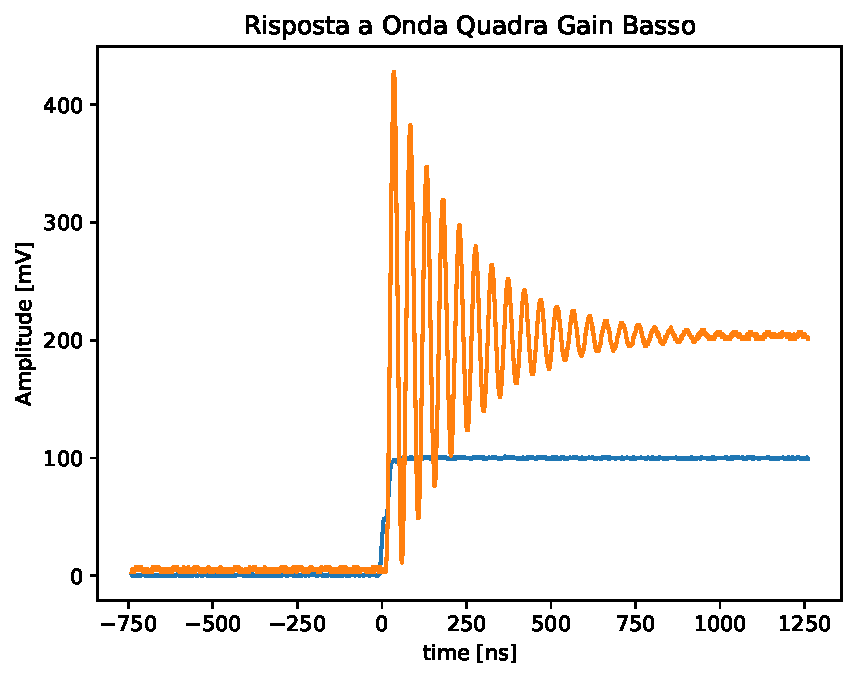
\includegraphics[width=.8\linewidth]{assets/AD848/Non Invertente/Non_inv_low_gain.pdf}
        \caption{Andamento oscillante a gain basso, (\href{https://github.com/Yedi278/Esperimentazioni-Elettronica/tree/main/-\%20OPAMP/AD848/Non-Invertente/R1\%202.2k\%20R2\%202.2k}{link dati})}
    \end{minipage}
    \begin{minipage}{0.5\linewidth}
        \centering
        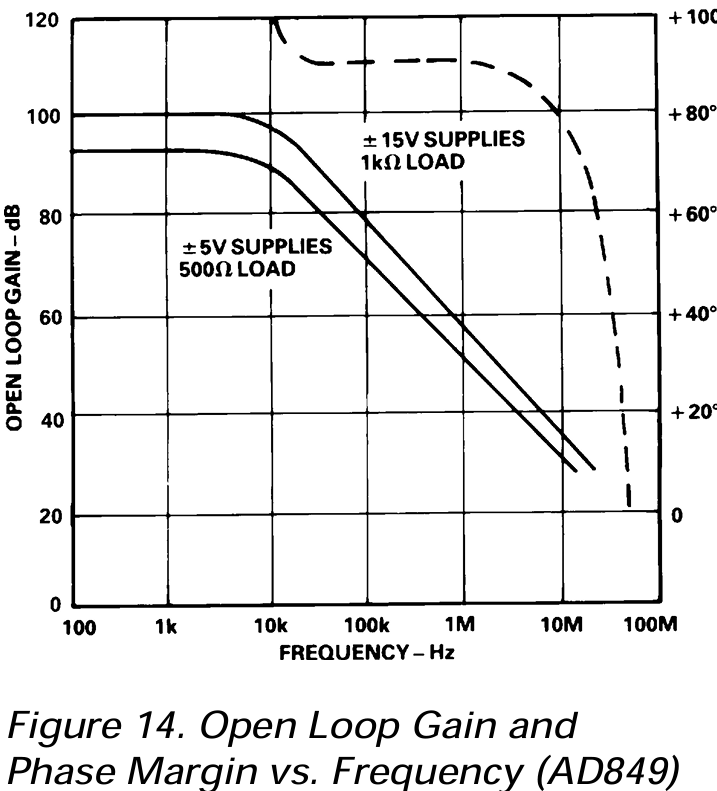
\includegraphics[width=.6\linewidth]{assets/AD848/AD848_PhaseMargin.png}
        \caption{Margine di fase AD848}
    \end{minipage}
\end{figure}

\begin{wrapfigure}[14]{r}{.5\linewidth}
    \centering
    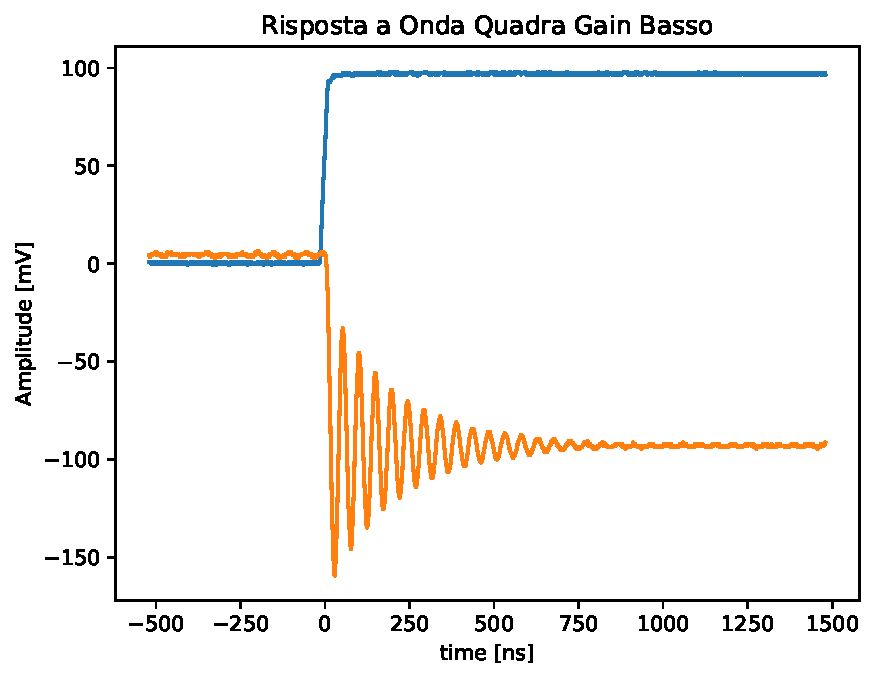
\includegraphics[width=\linewidth]{assets/AD848/Invertente/Inv_low_gain.pdf}
    \caption{AD848 Configurazione invertente a gain basso, (\href{https://github.com/Yedi278/Esperimentazioni-Elettronica/tree/main/-\%20OPAMP/AD848/Invertente/R1\%202.2k\%20R2\%202.2k\%20Instabilit\%C3\%A0/Quadra}{link dati})}
\end{wrapfigure}

$$$$
\'E possibile facilmente notare che in questa zona l'amplificatore non si comporta in maniera corretta; infatti, guardando il margine di frequenza, si nota che questo tende a 0° nella zona sotto 5 Gain ($\sim 13 dB$) rendendo il segnale di uscita totalmente inutilizzabile.

Nella configurazione invertente invece selezionando le stesse resistenze $R_1 = 2.2k\Omega$ e $R_2 = 2.2k\Omega$ è possibile ottnere un gain di -1 con il seguente andamento:


Come nel caso di configurazione non invertente il margine di fase risulta essere troppo basso e si ottiene instabilità evidente.

\pagebreak
\subsubsection{Gain elevato}

A gain superiore a 5 sono state prese misure sia in configurazione invertente che configurazione non invertente utilizzando un'onda quadra e resistenze $R_1 = 2.2k\Omega$ e $R_2 = \{ 14.7k\Omega, 31.5k\Omega, 48.5k\Omega \}$

\begin{figure}[!h]
    \centering
    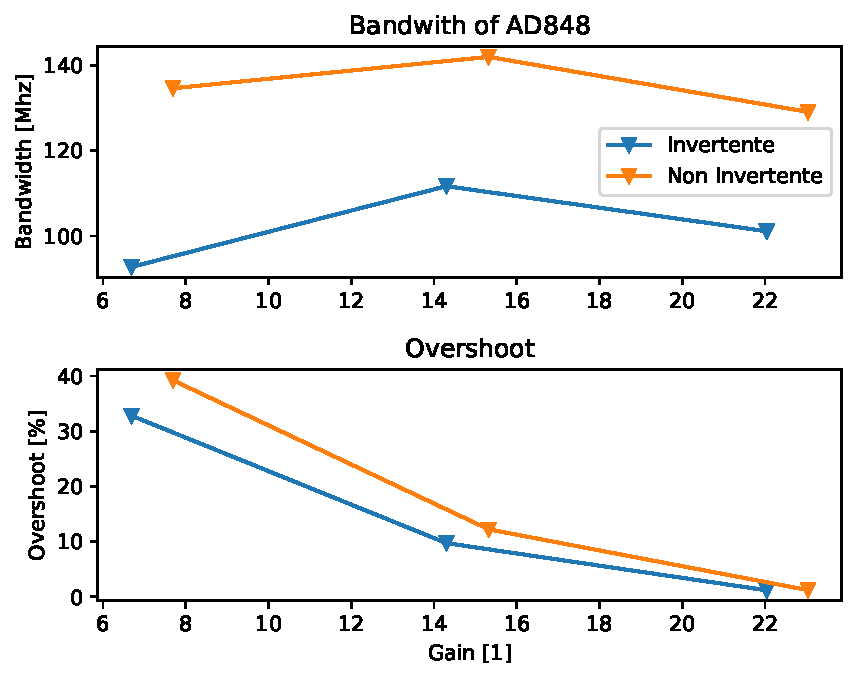
\includegraphics[width=0.5\linewidth]{assets/AD848/AD848_dati_tot.pdf}
    \caption{Andamento finale AD848 }
\end{figure}

Il valor medio di bandwith calcolato è \textbf{BW = 118.5 ± 17.9 MHz}.

\subsubsection{Conclusioni}
La presenza del doppio polo porta a un margine di fase molto ridotto a Gain basso ed instabilità del segnale che lo rende inutilizzabile. A Gain superiore alla soglia consigliata si ottiene un andamento consono e una bandwidth di \textbf{BW = 118.5 ± 17.9 MHz} in accordo con i datasheet.
Questo amplificatore permette guadagni molto più elevati dell' OP27 che permette di amplificare maggiormente il segnale del rilevatore a nostro vantaggio.

\pagebreak
\subsection{SiPm}
La parte finale della caratterizzazione della scheda richiede lo studio del rilevatore al suo interno, ovvero un SiPm (Silicon Photo Multiplier).

Questo rilevatore presenta al suo interno il sistema composto da SPAD e resistenze di quenching che permette la creazione di valanghe di elettroni controllate all'interno del rilevatore fino ad ottenere una risoluzione al singolo fotone.

\subsubsection{Setup}

Siccome la tensione generata dal SiPm è troppo bassa per la risoluzione dell'ADC è necessario applicare gli stadi di amplificazione studiati nei punti seguenti come mostrato in figura:

\begin{figure}[!h]
    \centering
    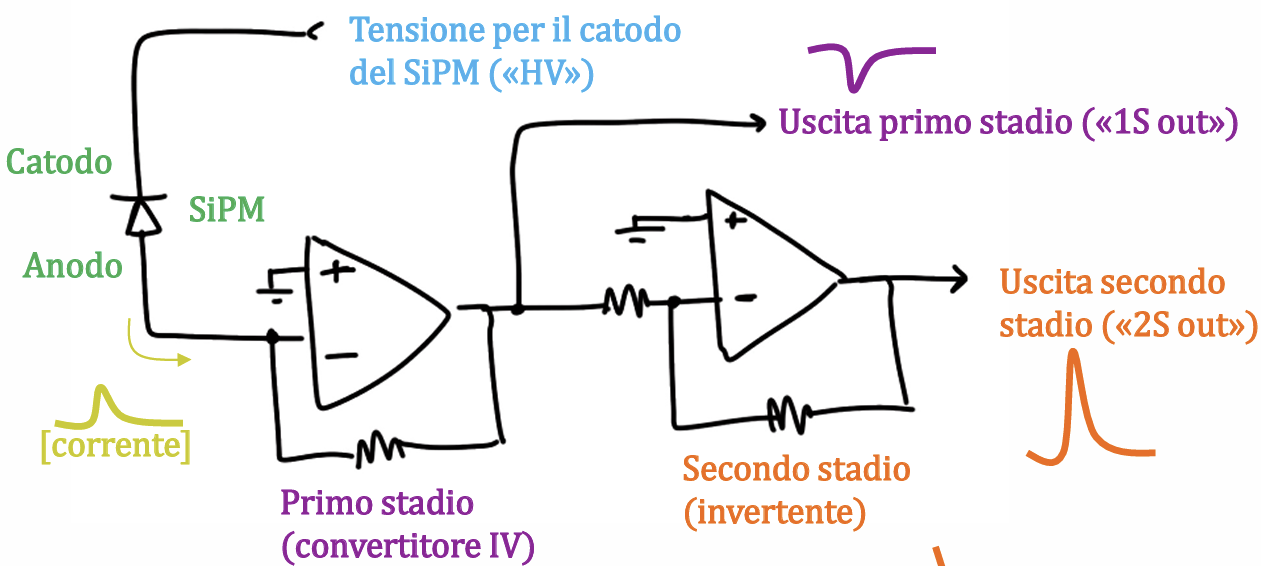
\includegraphics[width=0.5\linewidth]{assets/SiPm/SiPm_Stadi_Amp.png}
    \caption{Stadi di amplificazione}
    \label{fig:SiPm stadi di amp}
\end{figure}

Siccome i tempi di esistenza del segnale sono molto bassi, nell'ordine dei 100-200ns, risulta difficile ottenere una misurazione accurata con l'ADC che è limitato a campionamenti nell'ordine dei 200ns. Per questo è stato usato un sistema di Peak Hold:

\begin{figure}[!h]
    \centering
    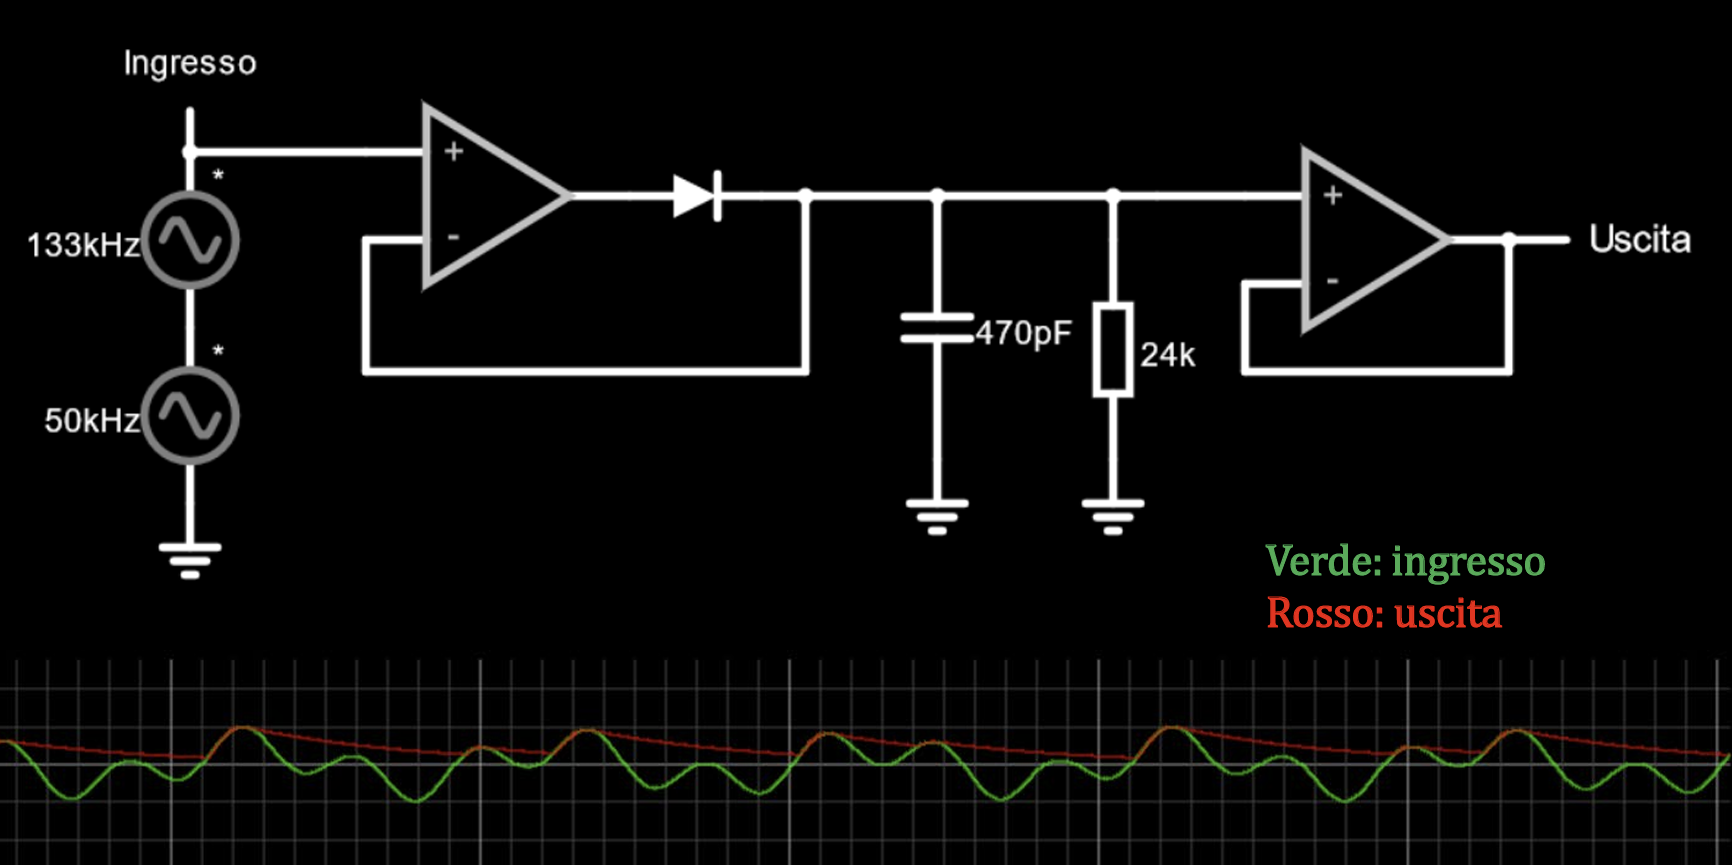
\includegraphics[width=0.5\linewidth]{assets/SiPm/SiPm_Peak_hold.png}
    \caption{Sistema di Peak Hold}
\end{figure}

All'uscita del peak hold la tensione viene mantenuta per un tempo sufficiente per l'acquisizione dell'ADC.

Come mostrato in figura \ref{fig:SiPm stadi di amp}, il rilevatore che si comporta come diodo è inserito in polarizzazione inversa nella scheda in maniera tale da sfruttarne la tensione di breakdown. Per comprendere la polarizzazione, è stata impostata inizialmente sull'alimentatore una tensione bassa e corrente limitata per controllare la polarizzazione corretta. Avendo inserito nei suoi pin la fonte luminosa a LED, è stata sigillata la zona contenente fonte luminosa e rilevatore. Successivamente, la tensione fornita al SiPm è stata portata a +3V di Overvoltage per permettere l'avvento della valanga di elettroni nello SPAD.

Fornendo al LED una tensione impulsata di 100 ns a circa 3.4 V è stato possibile osservare la rilevazione dei fotoni:

\begin{figure}[!h]
    \centering
    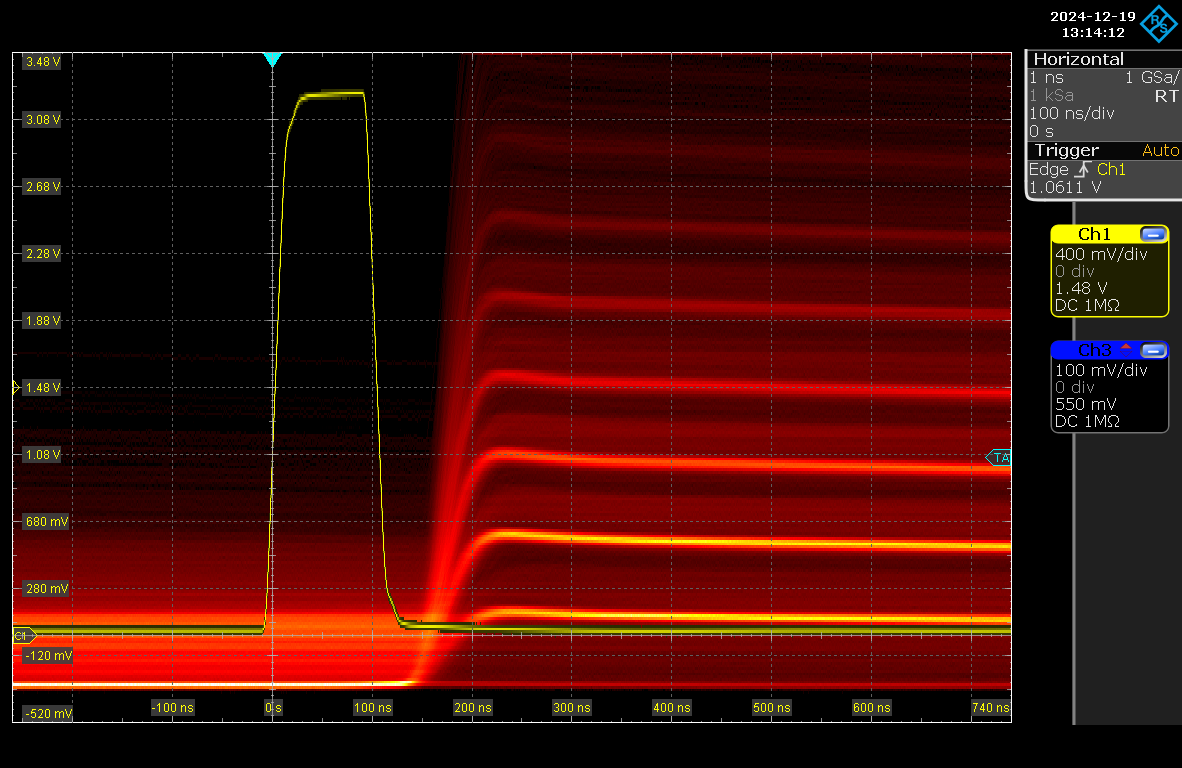
\includegraphics[width=0.5\linewidth]{assets/SiPm/SiPm.png}
    \caption{Prima visualizzazione dei segnali con persistance di 2 sec}
\end{figure}

E evidente la presenza di diverse zone con elevata densità di rilevazioni
che corrispondono a 1 fotone, 2 fotoni, 3 fotoni etc...

\subsubsection{Dark Count Rate}
Siccome gli elettroni nello spad sono soggetti ad agitazione termica, è possibile che un elettrone riesca casualmente a liberarsi anche senza la presenza di un fotone, portando a una valanga non desiderata. Questo è noto come DCR (Dark Count Rate).

Per caratterizzare il SiPm è utile avere una stima di questo fenomeno. Per questo è stato impostato l'oscilloscopio in modalità di conteggio dei segnali in arrivo. Impostata una soglia di trigger di circa mezzo fotone è stata fatta partire la misura di tempo per 40000 segnali a tensioni di overvoltage differenti.

\begin{figure}[!h]
    \centering
    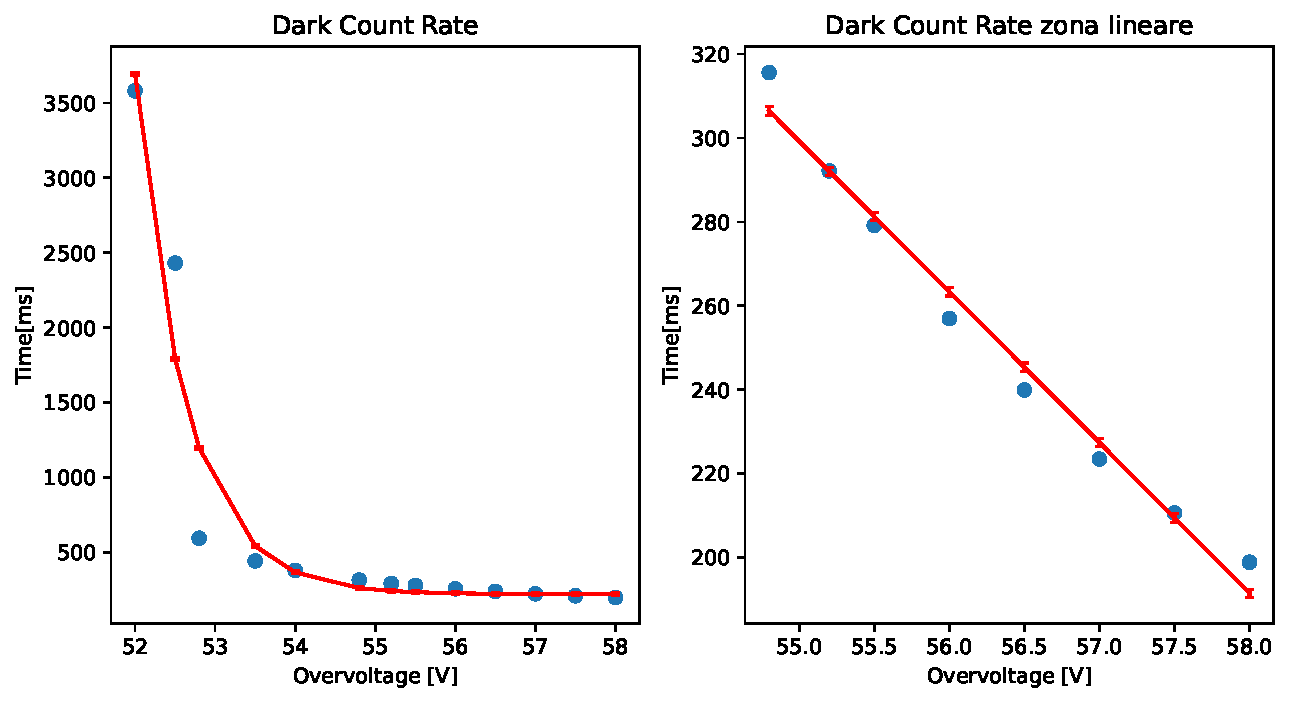
\includegraphics[width=0.6\linewidth]{assets/SiPm/SiPm_DCR.pdf}
    \caption{Tempi per conteggio di 40000 eventi, (\href{https://github.com/Yedi278/Esperimentazioni-Elettronica/tree/main/SiPm/Caratterizzazione\%20Hamamatsu}{link dati})}
\end{figure}

Nella zona prossima alla tensione di \textit{break down} il rate risulta molto basso, si suppone dovuto alla mancanza di campo elettrico fornito agli elettroni che non sono in grado in certi casi di produrre la valanga. Per tenisoni prossime a quelle di \textit{overvoltage} consigliate, ovvero $V_{OV} = 54.9V$, il rate si comporta in maniera approssimativamente lineare. Siccome il rate cambia di circa 31 ms/V possiamo approssimare questo rate ad un valore costante di circa \textbf{DCR = 158±38KHz}.
Questo valore risulta ragionevole con i valori inclusi nel manuale.

\section{Risultati}
Inserisci qui i risultati.

\section{Conclusioni}
Inserisci qui le conclusioni.

\end{document}